\documentclass[11pt]{article}

\usepackage[utf8]{inputenc}
\usepackage[T1]{fontenc}
\usepackage[spanish,es-nodecimaldot]{babel}
\usepackage{lmodern}
\usepackage{amsmath,amssymb}
\usepackage{booktabs}
\usepackage{array}
\usepackage{graphicx}
\usepackage{xcolor}
\usepackage{geometry}
\usepackage{microtype}
\usepackage{enumitem}
\usepackage{caption}
\usepackage{float}
\usepackage[hidelinks]{hyperref}

\geometry{margin=2.5cm}
\setlength{\parindent}{0pt}
\setlength{\parskip}{0.65em}
\setlist[itemize]{topsep=0.25em,itemsep=0.2em}
\captionsetup{font=small,labelfont=bf}

\definecolor{azul}{HTML}{1D4ED8}
\definecolor{gris}{HTML}{475569}
\definecolor{fondo}{HTML}{F1F5F9}

\newcommand{\E}{\mathbb{E}}
\newcommand{\Prob}{\mathbb{P}}
\newcommand{\BetaDist}{\operatorname{Beta}}
\newcommand{\idea}[1]{%
  \begin{center}
  \fcolorbox{gris}{fondo}{\begin{minipage}{0.91\textwidth}
  \textbf{Idea principal.} #1
  \end{minipage}}
  \end{center}}

\hypersetup{
  pdftitle={Modular DP: guía simple de los experimentos},
  pdfauthor={Reporte del perfil numérico full},
  pdfsubject={Métodos de aprendizaje, demanda y elección dinámica de calidad}
}

\title{\textbf{Modular DP: guía simple de los experimentos}\\[0.4em]
\large Aprendizaje, demanda y elección de calidad}
\author{Reporte basado en el perfil numérico \texttt{full}}
\date{\today}

\begin{document}

\maketitle

\begin{abstract}
Este reporte explica, con palabras y notación sencillas, los experimentos de
\texttt{Modular DP}. El objetivo es entender cómo distintas reglas de
aprendizaje cambian la demanda del vendedor A y, con ello, su incentivo para
usar un producto costoso pero de mayor calidad. Primero se presenta el modelo
común; después se describen Thompson sampling, actualizaciones escaladas,
temperatura, epsilon-greedy y olvido. Finalmente se resumen el programa
dinámico, las simulaciones, los principales resultados y sus limitaciones.
\end{abstract}

\tableofcontents
\newpage

\section{La pregunta económica}

Hay dos vendedores. El vendedor B ofrece una calidad conocida, denotada por
$p_0$. El vendedor A tiene una reputación que los usuarios aprenden a partir
de resultados binarios: éxito o fracaso.

Cuando A recibe una interacción, elige en privado entre dos productos:

\begin{center}
\begin{tabular}{lccc}
\toprule
Producto & Probabilidad de éxito & Costo & Ganancia inmediata \\
\midrule
1: barato & $p_1=0.35$ & $c_1=0.05$ & $R-c_1=0.95$ \\
2: alta calidad & $p_2=0.80$ & $c_2=0.65$ & $R-c_2=0.35$ \\
\bottomrule
\end{tabular}
\end{center}

El ingreso es $R=1$. El producto 1 deja más ganancia hoy, pero el producto 2
produce éxitos con mayor frecuencia y puede mejorar la reputación de A. La
empresa valora el futuro con factor de descuento $\gamma=0.98$.

La pregunta central es:

\idea{¿Durante cuánto tiempo vale la pena sacrificar ganancia presente para
mejorar la reputación y atraer demanda futura?}

Todos los experimentos mantienen este problema del vendedor. Lo que cambia es
la regla mediante la cual el usuario convierte la evidencia observada en una
probabilidad de elegir A.

\section{Creencias y demanda}

\subsection{La creencia básica}

Sea $S$ el número de éxitos observados y $F$ el número de fracasos. Se parte de
una distribución uniforme $\BetaDist(1,1)$. Después de observar $(S,F)$, la
creencia estándar es
\begin{equation}
  \theta\mid S,F \sim \BetaDist(1+S,1+F),
\end{equation}
donde $\theta$ representa la calidad desconocida de A. Su media es
\begin{equation}
  m(S,F)=\frac{1+S}{2+S+F}.
\end{equation}

La notación que se usará en todo el reporte es:

\begin{center}
\begin{tabular}{>{\centering\arraybackslash}p{2.2cm}p{10.4cm}}
\toprule
Símbolo & Significado \\
\midrule
$S,F$ & Éxitos y fracasos observados para A. \\
$m$ & Calidad media que el usuario atribuye a A. \\
$p_0$ & Calidad conocida del vendedor B. \\
$D$ & Probabilidad de que el usuario elija A. \\
$V$ & Valor presente de las ganancias futuras de A. \\
$\eta,T,\varepsilon,\rho$ & Parámetros de los métodos alternativos. \\
\bottomrule
\end{tabular}
\end{center}

\subsection{Thompson sampling estándar}

Thompson sampling hace un sorteo $\widetilde\theta$ de la creencia y elige A
si el sorteo supera a $p_0$. Por tanto,
\begin{equation}
  D_{\mathrm{TS}}(S,F)
  =\Prob\!\left(\widetilde\theta\ge p_0\right),
  \qquad
  \widetilde\theta\sim\BetaDist(1+S,1+F).
\end{equation}

No significa que el usuario crea que A tiene exactamente esa probabilidad de
éxito. Significa que la demanda es la probabilidad de que una muestra de la
creencia de A supere a la opción conocida.

\section{Métodos comparados}

\subsection{Actualizaciones escaladas}

Las actualizaciones escaladas multiplican cada observación por $\eta$:
\begin{equation}
  \theta\mid S,F
  \sim \BetaDist(1+\eta S,\,1+\eta F).
\end{equation}

\begin{itemize}
  \item Si $\eta<1$, cada dato pesa menos y el prior tarda más en desaparecer.
  \item Si $\eta>1$, cada dato pesa más y el usuario reacciona con más fuerza.
  \item Si $\eta=1$, se recupera Thompson sampling estándar.
\end{itemize}

El experimento usa $\eta\in\{0.25,0.5,1,2,4\}$.

\subsection{Temperatura que preserva la media}

La temperatura modifica la concentración de la creencia sin cambiar su media:
\begin{equation}
  \theta\mid S,F
  \sim
  \BetaDist\!\left(\frac{1+S}{T},\frac{1+F}{T}\right).
\end{equation}
En efecto,
\begin{equation}
  \frac{(1+S)/T}{(2+S+F)/T}
  =\frac{1+S}{2+S+F}=m(S,F).
\end{equation}

Así, $T$ cambia la incertidumbre pero no la estimación media:
\begin{itemize}
  \item $T<1$: distribución más concentrada, como si hubiera más precisión.
  \item $T>1$: distribución más dispersa, como si hubiera menos precisión.
  \item $T=1$: Thompson sampling estándar.
\end{itemize}

El experimento usa $T\in\{0.25,0.5,1,2,4\}$.

\subsection{Epsilon-greedy uniforme}

Epsilon-greedy compara la media $m$ con $p_0$. Con probabilidad
$1-\varepsilon$ el usuario toma la opción con mayor media; con probabilidad
$\varepsilon$ explora uniformemente entre A y B. La demanda de A es
\begin{equation}
D_{\varepsilon}(m)=
\begin{cases}
1-\varepsilon/2, & m>p_0,\\
1/2, & m=p_0,\\
\varepsilon/2, & m<p_0.
\end{cases}
\end{equation}

Por ejemplo, si $\varepsilon=0.1$, la demanda puede ser $0.95$, $0.50$ o
$0.05$. Esta es exploración uniforme entre dos vendedores; no es la versión
de exploración dirigida que asigna toda la exploración a A.

El experimento usa
$\varepsilon\in\{0,0.02,0.05,0.1,0.2,0.5,1\}$.

\subsection{Olvido}

Para explicar el olvido conviene usar dos contadores efectivos, $u$ para
éxitos y $v$ para fracasos. La creencia es
\begin{equation}
  \theta\sim\BetaDist(1+u,1+v).
\end{equation}

Cuando llega una observación nueva, una fracción $\rho$ de la evidencia vieja
se conserva:
\begin{align}
  \text{éxito:}\quad &(u',v')=(\rho u+1,\rho v),\\
  \text{fracaso:}\quad &(u',v')=(\rho u,\rho v+1).
\end{align}

Cuanto más pequeño es $\rho$, más rápido se olvida. Se comparan dos relojes:

\begin{itemize}
  \item \textbf{Olvido por observación:} si B es elegido, no cambia la memoria,
  $(u',v')=(u,v)$.
  \item \textbf{Olvido por calendario:} la memoria envejece cada periodo, aun
  cuando B es elegido, $(u',v')=(\rho u,\rho v)$.
\end{itemize}

La memoria efectiva está acotada aproximadamente por
\begin{equation}
  u+v\le \frac{1}{1-\rho}.
\end{equation}
Esta cota es la diferencia esencial con los métodos de conteos acumulados: el
pasado nunca llega a dominar completamente a la información reciente.

\section{El problema dinámico del vendedor}

Sea $z$ el estado actual de la creencia. Escribimos $z^+$ para el estado tras
un éxito, $z^-$ tras un fracaso y $z^0$ cuando A no es elegido. Si A usa el
producto $j\in\{1,2\}$, su valor condicional a recibir la interacción es
\begin{equation}
  Q_j(z)=R-c_j+\gamma\big[p_jV(z^+)+(1-p_j)V(z^-)\big].
\end{equation}

La ecuación de Bellman es
\begin{equation}
  V(z)=D(z)\max\{Q_1(z),Q_2(z)\}
  +\gamma[1-D(z)]V(z^0).
  \label{eq:bellman}
\end{equation}

La primera parte corresponde a periodos en que A es elegido. La segunda parte
corresponde a periodos sin venta para A.

La diferencia entre los dos productos se simplifica a
\begin{equation}
Q_2(z)-Q_1(z)
=-(c_2-c_1)
+\gamma(p_2-p_1)\big[V(z^+)-V(z^-)\big].
\end{equation}

Por tanto, el producto 2 es óptimo si
\begin{equation}
  \gamma\big[V(z^+)-V(z^-)\big]
  >\frac{c_2-c_1}{p_2-p_1}
  =\frac{0.60}{0.45}=\frac{4}{3}.
  \label{eq:threshold}
\end{equation}

El lado izquierdo mide cuánto vale conseguir un éxito en lugar de un fracaso.
El lado derecho es el costo adicional por unidad adicional de probabilidad de
éxito.

Cuando $z^0=z$, como sucede en todos los métodos de conteos y en el olvido por
observación, la ecuación~\eqref{eq:bellman} puede despejarse exactamente:
\begin{equation}
  V(z)=
  \frac{D(z)\max\{Q_1(z),Q_2(z)\}}
       {1-\gamma[1-D(z)]}.
\end{equation}
Para el olvido por calendario no se puede hacer este despeje porque la
creencia cambia incluso cuando A no es elegido.

\section{Qué experimentos se realizaron}

\subsection{Sensibilidad de la demanda}

Para un estado con $n=S+F$ observaciones se calcula cuánto cambia la demanda
si la próxima observación es un éxito en vez de un fracaso:
\begin{equation}
  g_n=\max_{S+F=n}
  \left[D(S+1,F)-D(S,F+1)\right].
\end{equation}

Si $g_n$ cae hacia cero, una observación adicional termina teniendo muy poco
efecto sobre la demanda. Si la sensibilidad permanece grande, todavía puede
haber un incentivo reputacional para usar alta calidad.

\begin{figure}[H]
  \centering
  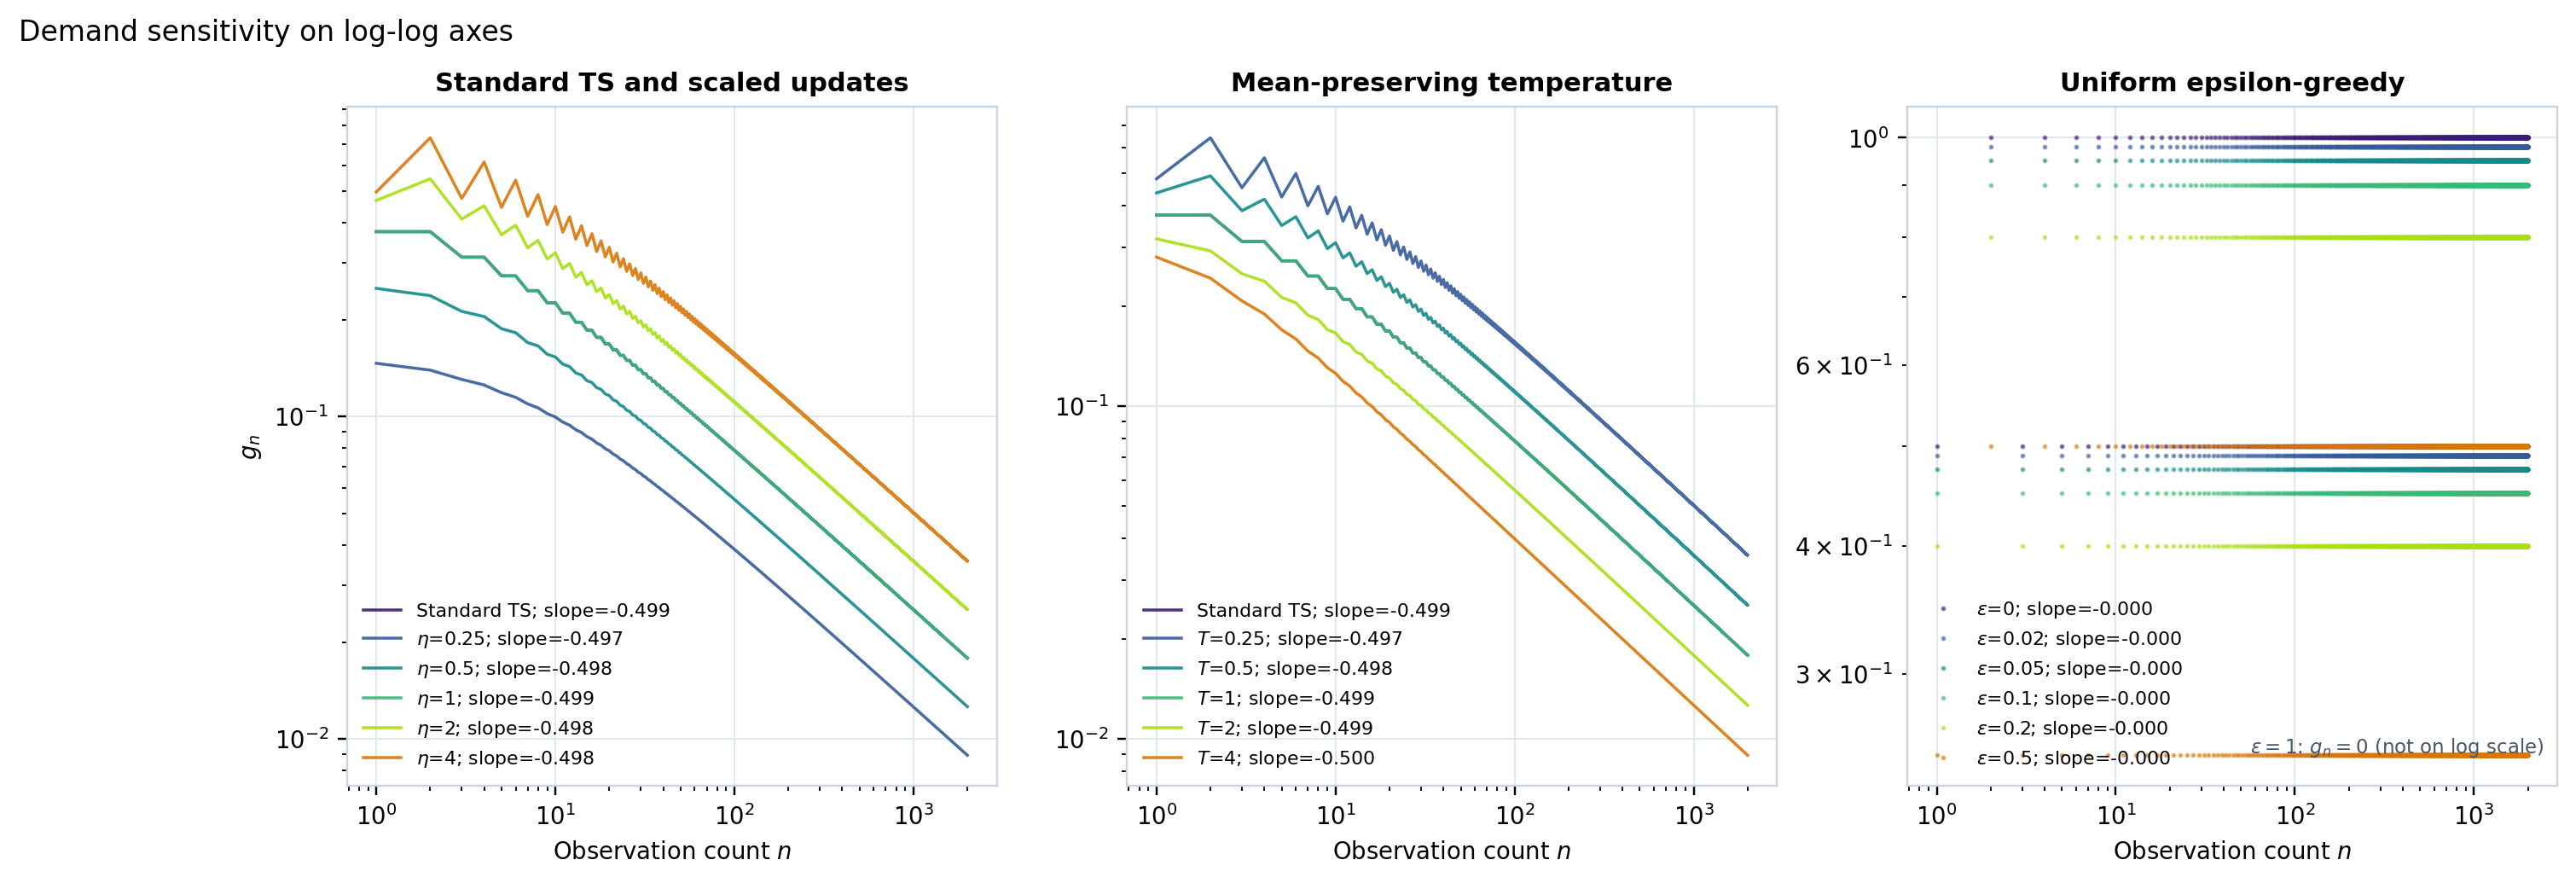
\includegraphics[width=0.98\textwidth]
    {../figures/full/demand/02_demand_sensitivity_loglog.png}
  \caption{Sensibilidad máxima de la demanda. Las reglas suaves de conteos se
  aproximan a la pendiente de referencia $-1/2$. Epsilon-greedy conserva un
  salto en el umbral y por eso no sigue la misma caída suave.}
  \label{fig:sensitivity}
\end{figure}

\subsection{Regiones de política}

Para cada estado se resuelve si el producto 1 o el producto 2 maximiza el
valor. Los gráficos muestran dónde la ventaja reputacional supera el costo
adicional de calidad.

\begin{figure}[H]
  \centering
  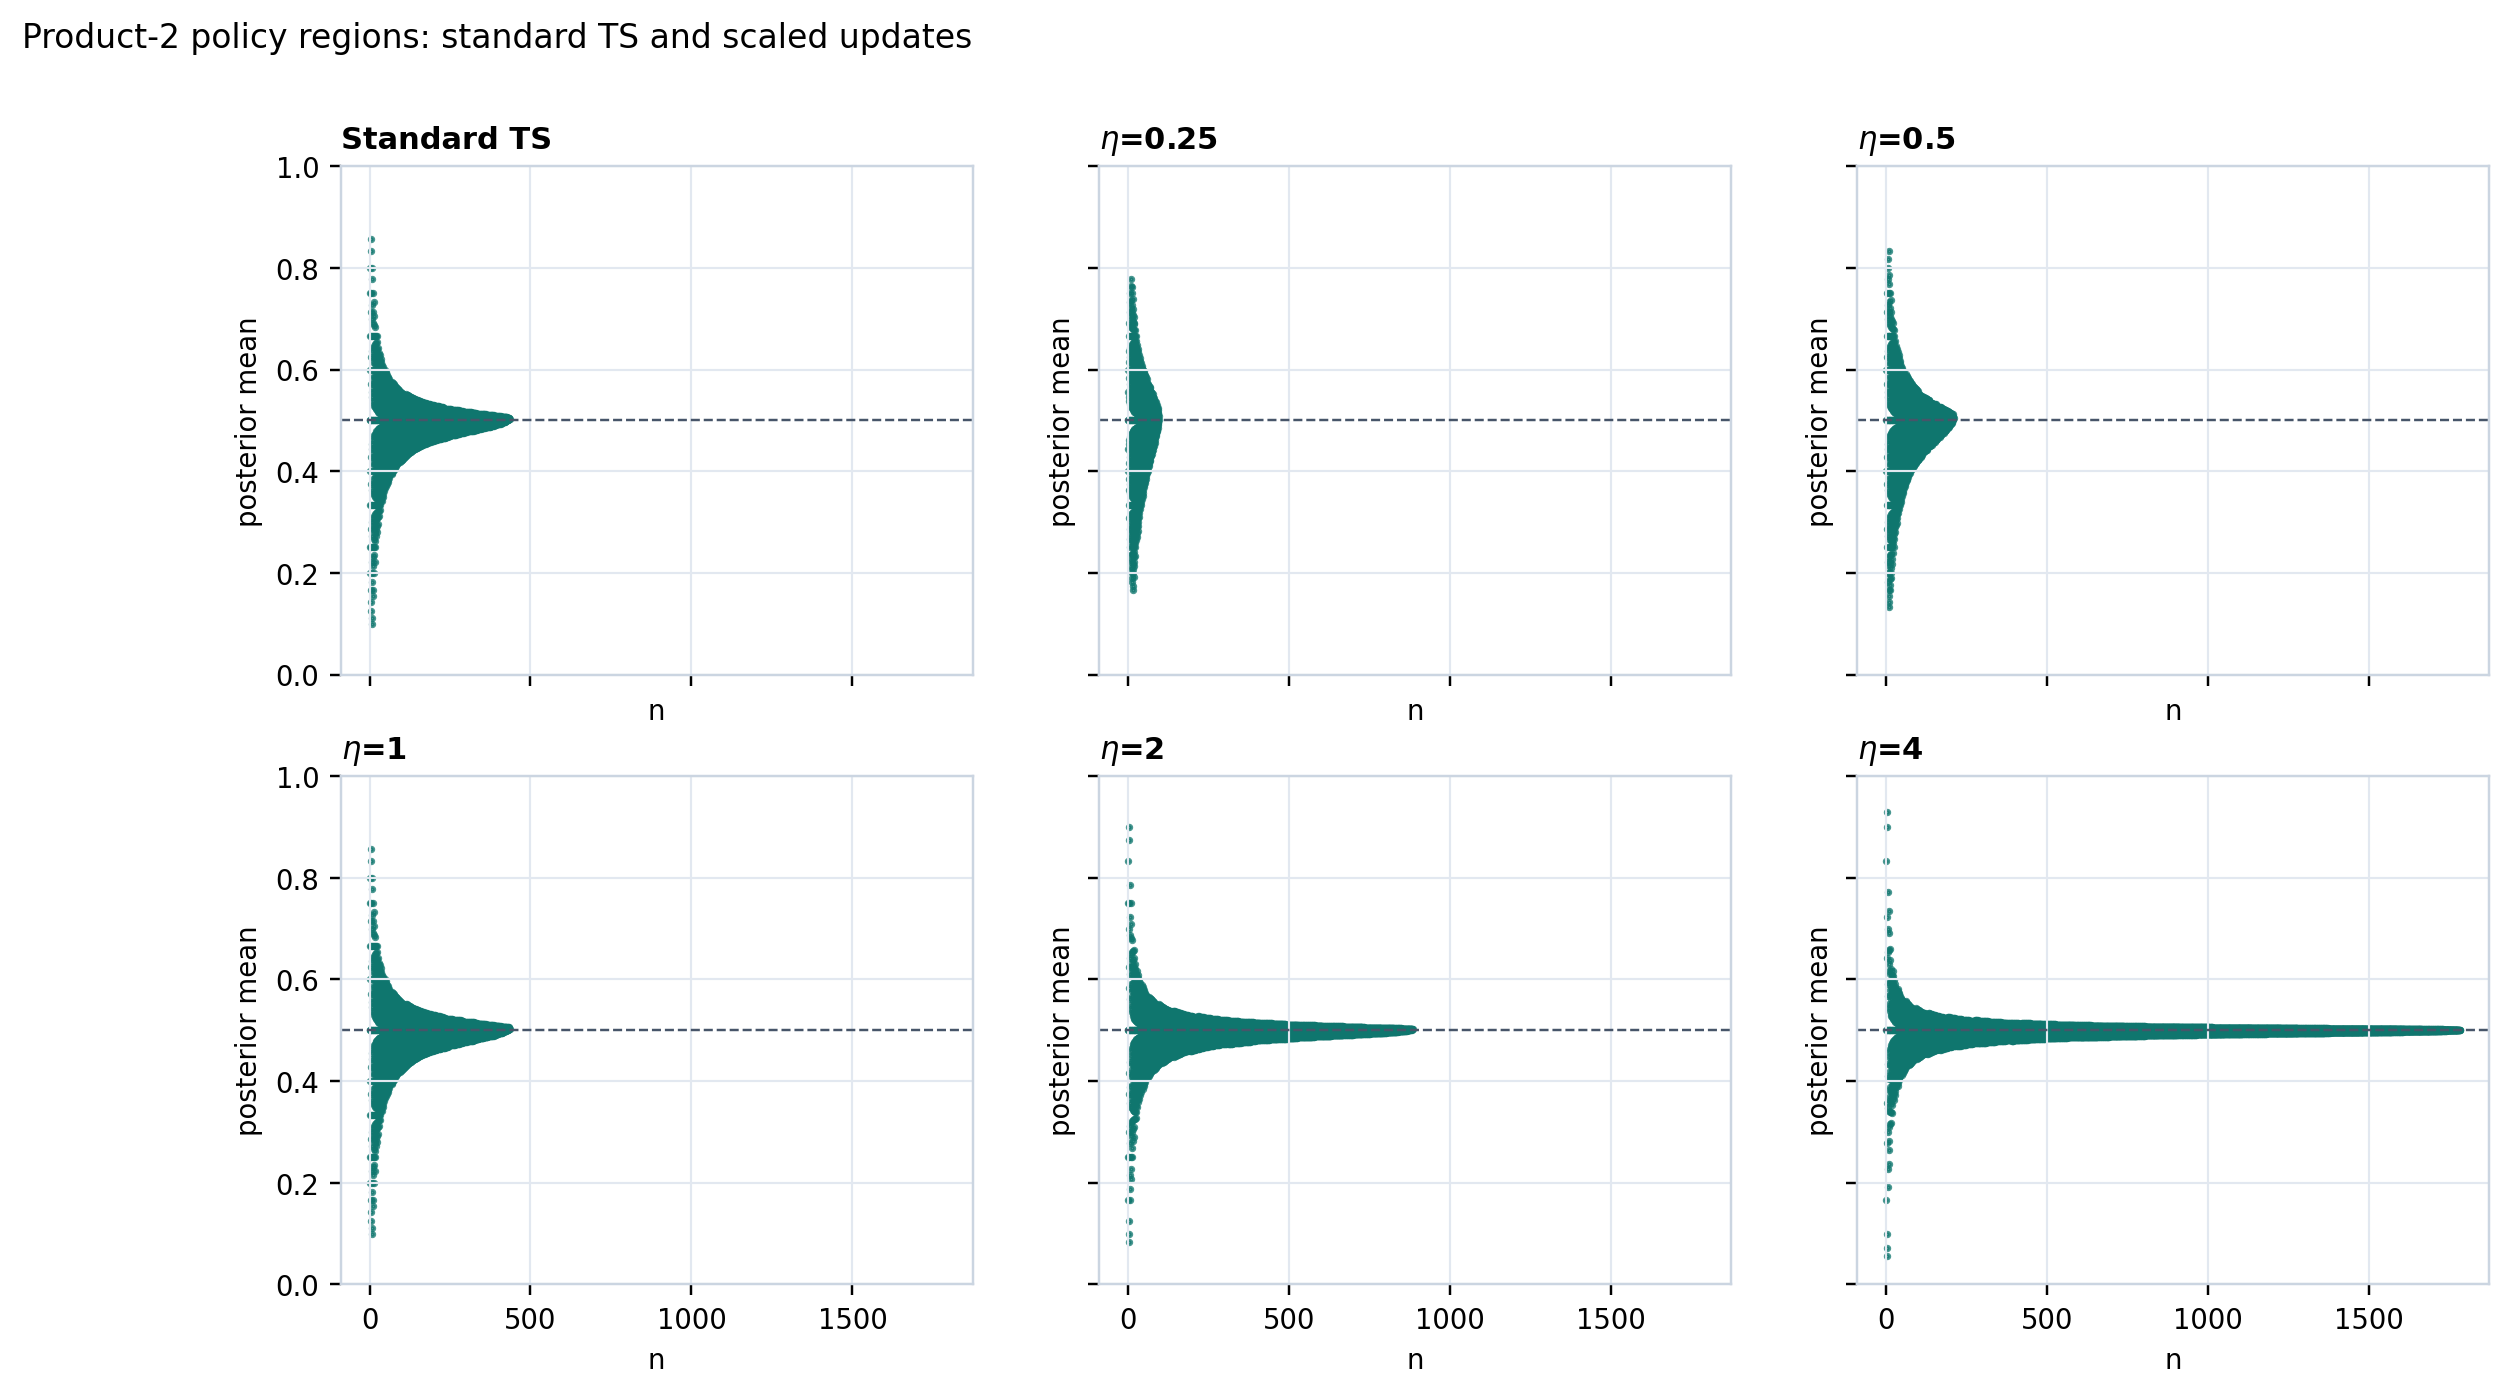
\includegraphics[width=0.98\textwidth]
    {../figures/full/policy/03_policy_standard_scaled.png}
  \caption{Regiones donde el producto 2 es óptimo bajo Thompson sampling y
  actualizaciones escaladas. El eje horizontal representa evidencia acumulada
  y el vertical resume la creencia media.}
  \label{fig:policy-scaled}
\end{figure}

\begin{figure}[H]
  \centering
  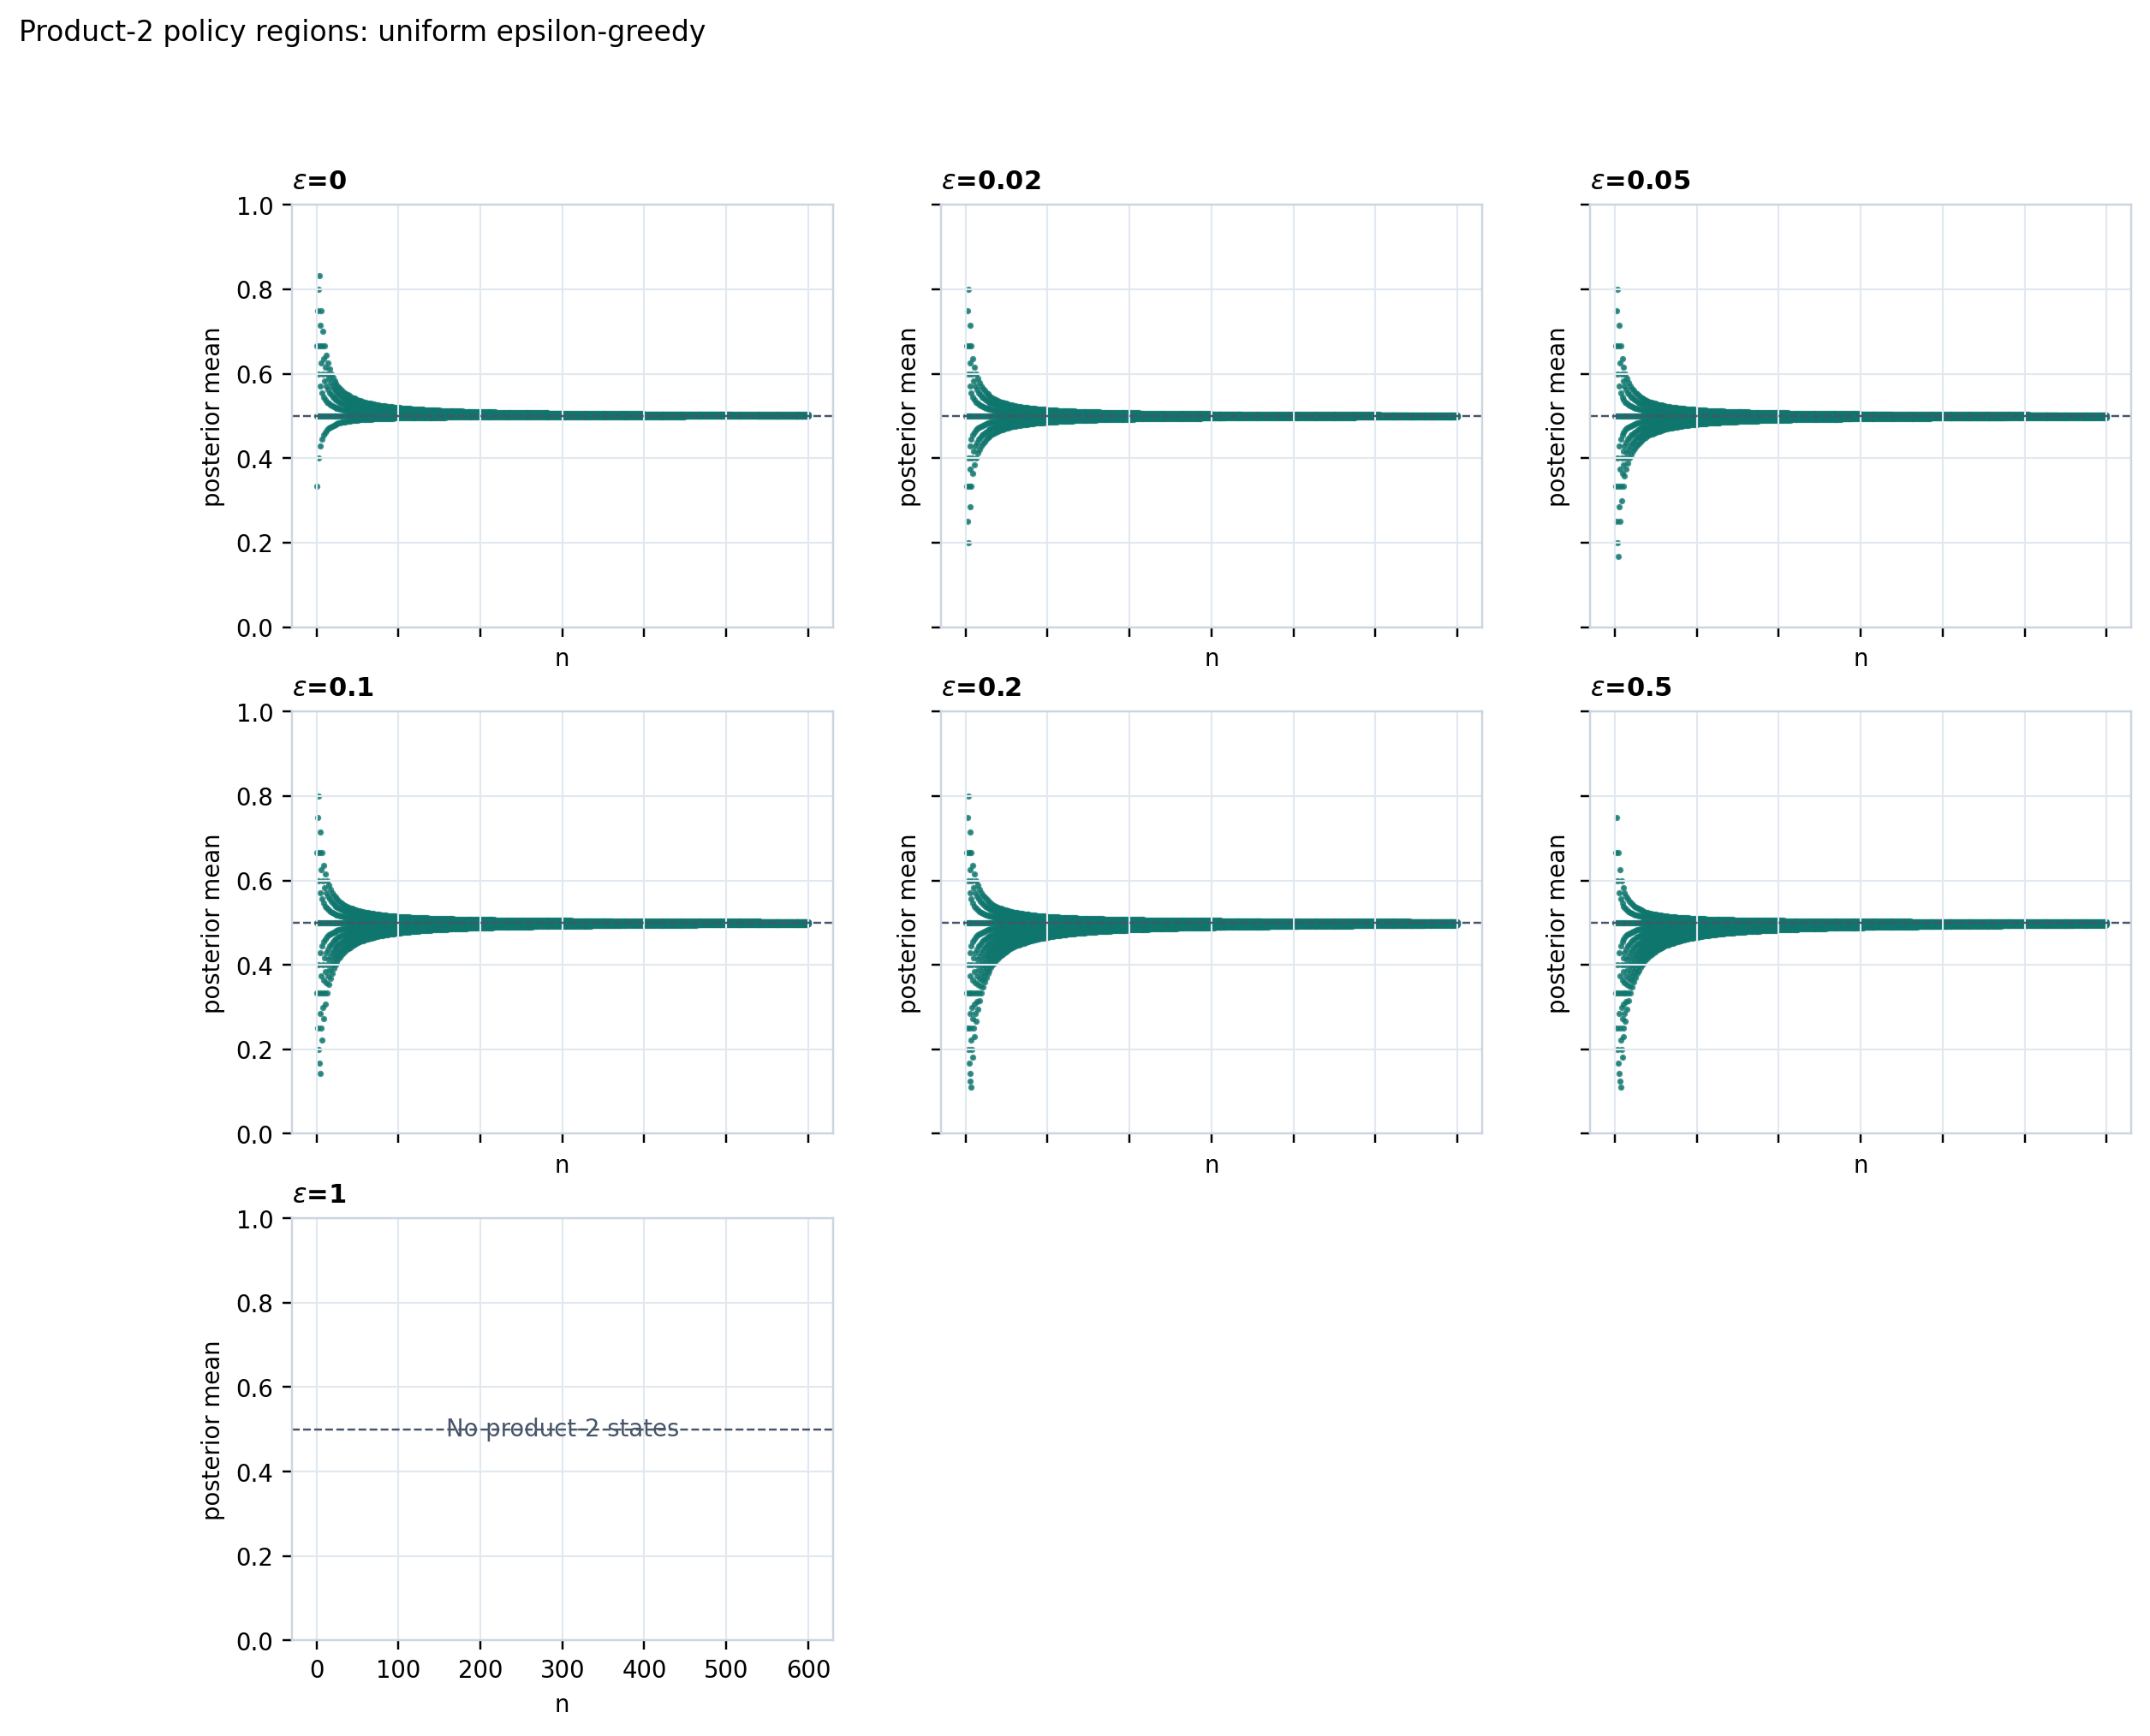
\includegraphics[width=0.98\textwidth]
    {../figures/full/policy/05_policy_epsilon_greedy.png}
  \caption{Regiones de producto 2 con epsilon-greedy uniforme. El salto de la
  demanda cerca de $m=p_0$ mantiene estados activos a niveles altos de
  evidencia para $\varepsilon<1$.}
  \label{fig:policy-epsilon}
\end{figure}

\subsection{Simulaciones largas}

El perfil completo simula 1,000 trayectorias durante 5,000 periodos, desde el
mismo prior y con números aleatorios comunes entre métodos. Se reportan, entre
otras cantidades, demanda, ganancia, uso de producto 2 y uso tardío en los
periodos 4,000 a 5,000.

\begin{center}
\small
\begin{tabular}{lrrr}
\toprule
Método & Demanda realizada & Uso tardío de 2 dado A & Ganancia descontada \\
\midrule
TS estándar & 0.132 & 0.000 & 27.03 \\
Escalado, $\eta=0.5$ & 0.093 & 0.000 & 25.01 \\
Escalado, $\eta=2$ & 0.218 & 0.000 & 28.24 \\
Temperatura, $T=0.5$ & 0.218 & 0.000 & 28.53 \\
Temperatura, $T=2$ & 0.093 & 0.000 & 25.32 \\
Epsilon-greedy, $\varepsilon=0.1$ & 0.922 & 0.334 & 28.77 \\
Olvido por observación, $\rho=0.95$ & 0.778 & 0.544 & 22.61 \\
Olvido por calendario, $\rho=0.95$ & 0.783 & 0.572 & 22.34 \\
\bottomrule
\end{tabular}
\end{center}

``Uso tardío de 2 dado A'' es la fracción de interacciones tardías de A en las
que efectivamente se empleó el producto 2. No es la fracción de todos los
periodos del calendario.

\begin{figure}[H]
  \centering
  \begin{minipage}[t]{0.49\textwidth}
    \centering
    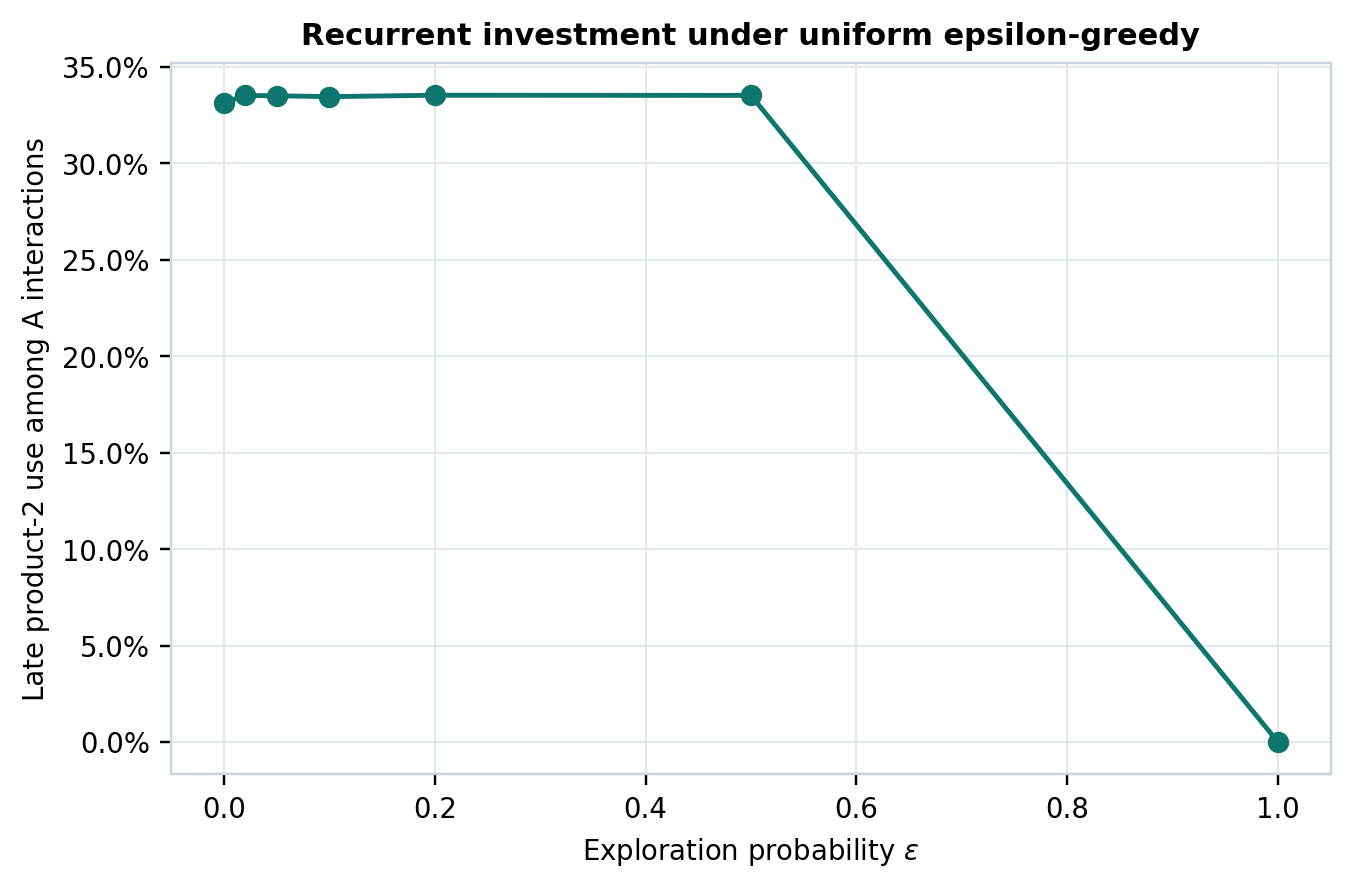
\includegraphics[width=\textwidth]
      {../figures/full/simulation/10_long_run_product2_vs_epsilon.png}
  \end{minipage}\hfill
  \begin{minipage}[t]{0.49\textwidth}
    \centering
    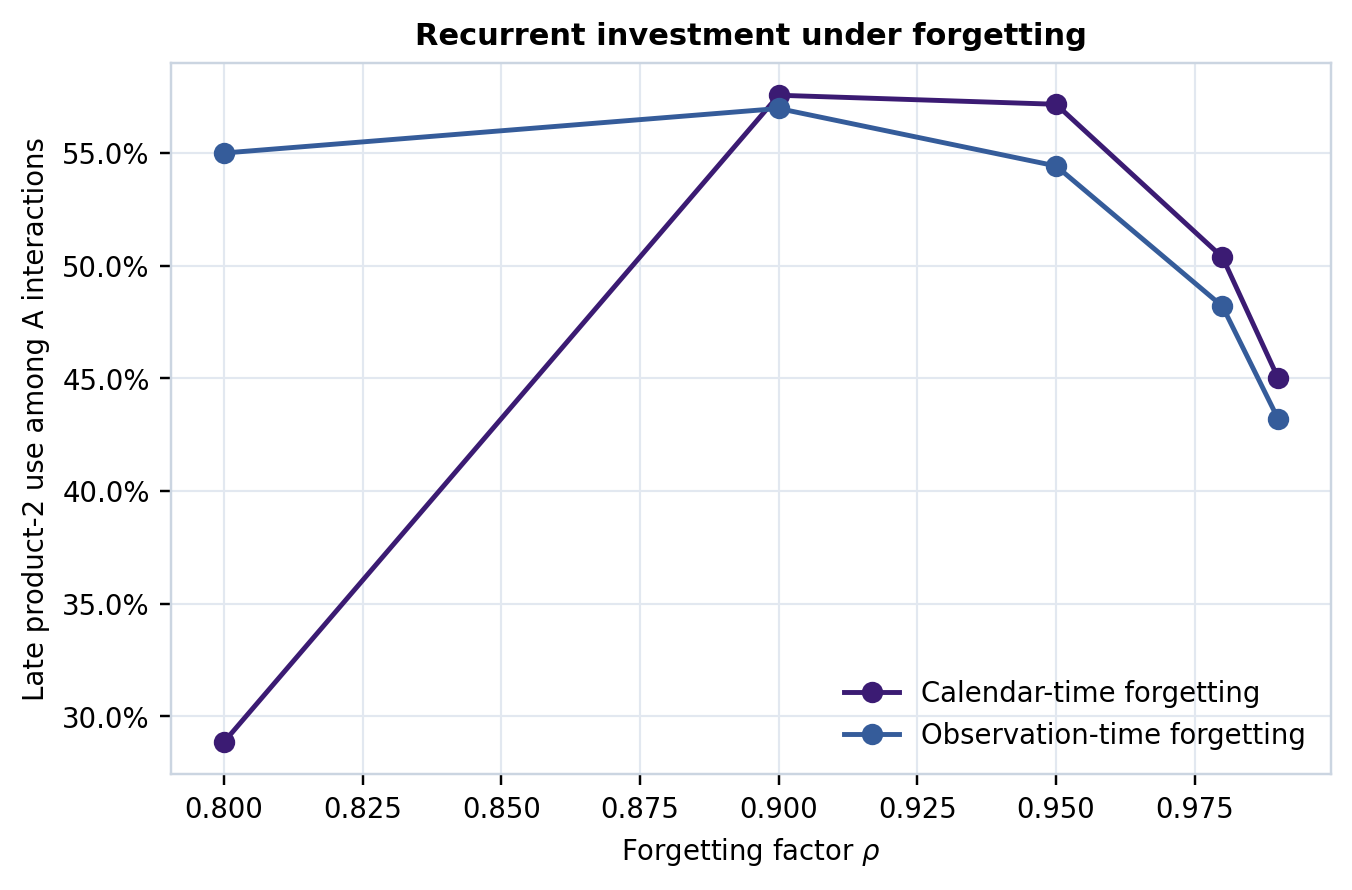
\includegraphics[width=\textwidth]
      {../figures/full/simulation/09_long_run_product2_vs_rho.png}
  \end{minipage}
  \caption{Uso tardío del producto 2 al variar exploración (izquierda) y
  memoria (derecha). Son diagnósticos dentro de un horizonte finito.}
  \label{fig:late-use}
\end{figure}

\subsection{Matriz dinámica para distintos valores de p0}

El segundo bloque de simulaciones cambia la calidad de la opción B:
\begin{equation}
  p_0\in\{0.1,0.3,0.5,0.7,0.9\}.
\end{equation}
Para cada valor se simulan 1,000 trayectorias durante 250 periodos. Cada panel
muestra promedios contemporáneos entre trayectorias, no promedios acumulados.

Como referencia se dibuja la mezcla mínima que iguala la calidad esperada de
B:
\begin{equation}
  a_{\mathrm{mant}}
  =\frac{p_0-p_1}{p_2-p_1},
\end{equation}
si el resultado está entre cero y uno. Para $p_0=0.5$ esta mezcla es
$a_{\mathrm{mant}}=1/3$. Es sólo un punto de comparación de calidad, no la
solución del programa dinámico.

\begin{figure}[H]
  \centering
  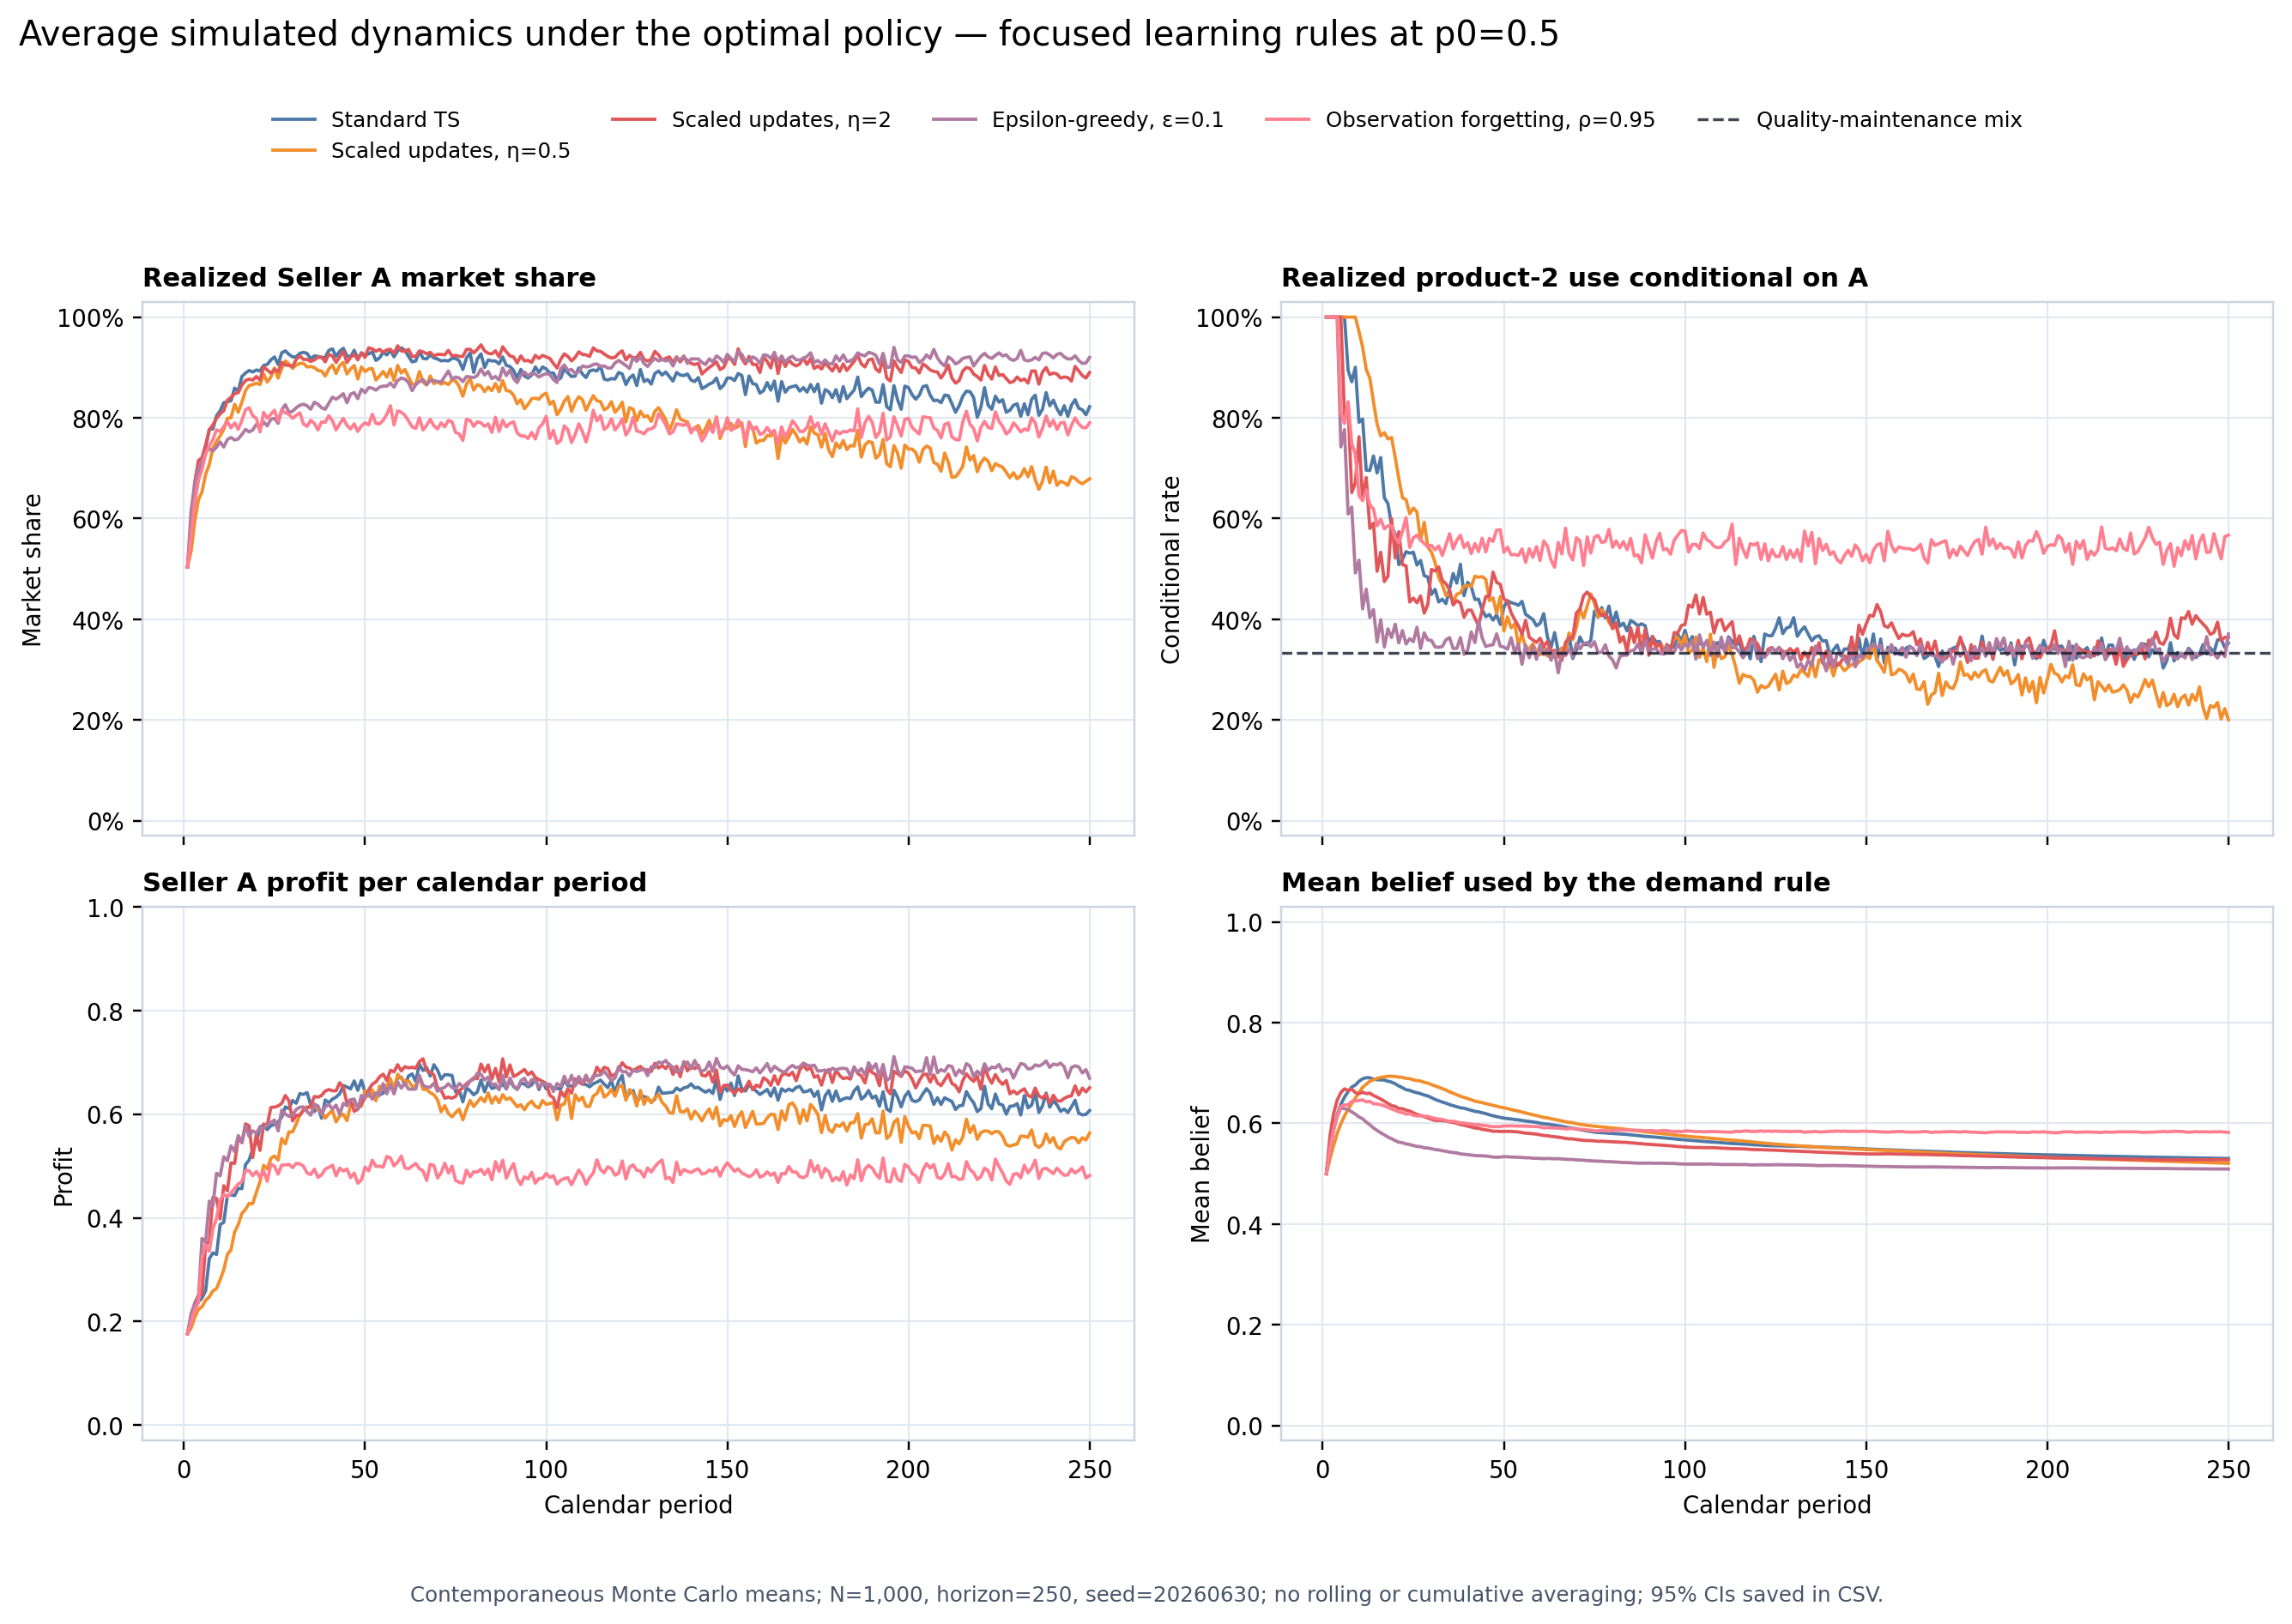
\includegraphics[width=0.98\textwidth]
    {../figures/full/dynamic/focused/20_dynamic_p0_0p5_focused_methods.png}
  \caption{Dinámica enfocada para $p_0=0.5$. Se muestran market share, uso
  efectivo del producto 2 condicional en A, ganancia y creencia media. Las
  diferencias al comienzo son transiciones; no deben confundirse con los
  resultados tardíos de la simulación de 5,000 periodos.}
  \label{fig:dynamic-p05}
\end{figure}

\section{Cómo se resolvió numéricamente}

\subsection{Estados discretos}

Los métodos sin olvido viven en la cuadrícula triangular
\begin{equation}
  (S,F),\qquad S\ge0,\quad F\ge0.
\end{equation}
El valor se calcula hacia atrás desde una diagonal exterior. El perfil completo
compara diagonales exteriores 800, 1,200 y 1,600 sobre el mismo interior
$S+F\le600$. Cuando la región activa queda demasiado cerca del borde, se usan
diagonales 3,000 y 3,600 y se compara hasta $S+F\le2,200$.

\subsection{Estados continuos de olvido}

Con olvido, $u$ y $v$ no son enteros. Para mantener una región numérica
acotada se usan las coordenadas
\begin{equation}
  x=(1-\rho)u,\qquad y=(1-\rho)v,
\end{equation}
que satisfacen $x\ge0$, $y\ge0$ y $x+y\le1$. El valor se calcula en una malla
triangular y se interpola linealmente entre nodos. Se comparan resoluciones
201, 401 y, para casos seleccionados, 801 o superiores.

\subsection{Validaciones}

Antes de cada corrida se ejecutan pruebas automáticas que verifican:
\begin{itemize}
  \item la ecuación de Bellman y sus residuos;
  \item acuerdo con el solver base;
  \item las identidades $\eta=1$ y $T=1$ con Thompson sampling estándar;
  \item estabilidad de la política al ampliar la frontera;
  \item transiciones e interpolación de los modelos con olvido;
  \item estabilidad sobre estados visitados en las simulaciones.
\end{itemize}

\begin{figure}[H]
  \centering
  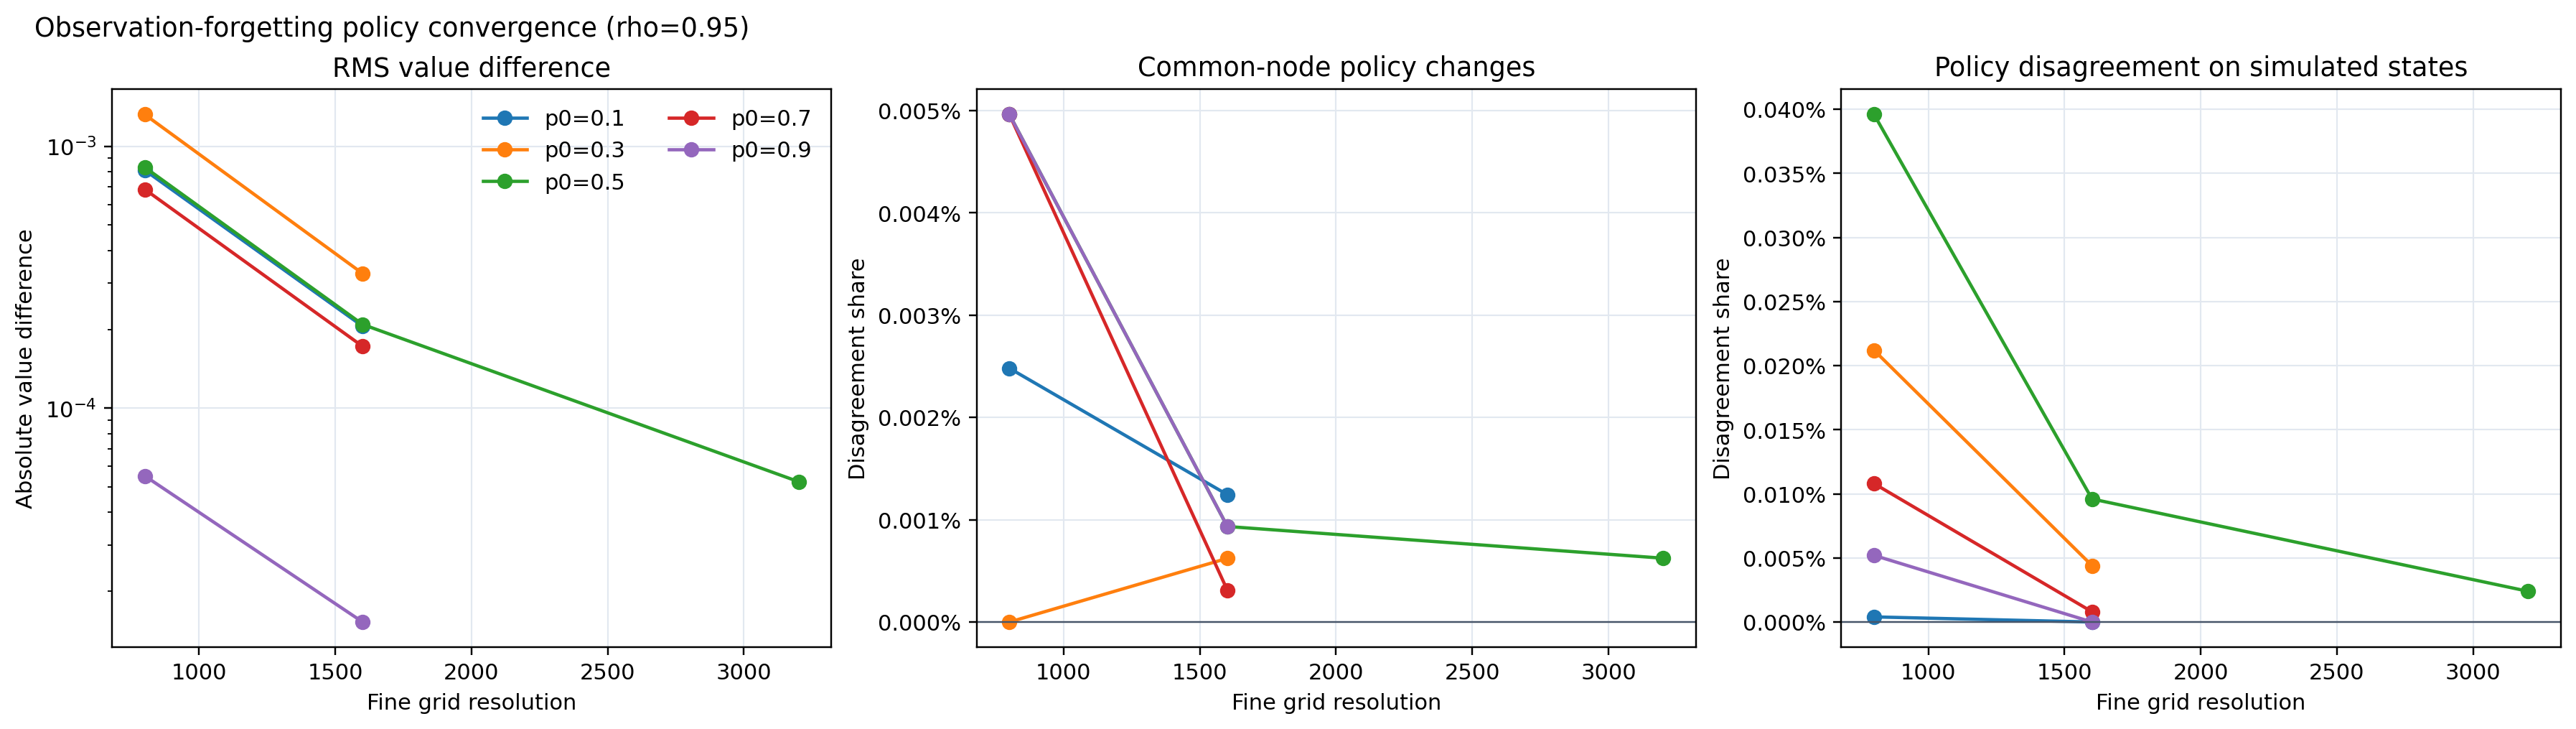
\includegraphics[width=0.96\textwidth]
    {../figures/full/diagnostics/23_observation_forgetting_convergence.png}
  \caption{Diagnóstico de convergencia para olvido por observación. El valor
  converge aproximadamente a segundo orden y los desacuerdos de política se
  concentran en una frontera muy delgada.}
  \label{fig:convergence}
\end{figure}

\section{Lectura simple de los resultados}

\subsection{Métodos de conteos acumulados}

Para Thompson sampling, actualizaciones escaladas y temperatura fija, la
sensibilidad marginal de la demanda se reduce a medida que crece la evidencia.
En la política numérica, la región de producto 2 termina después de una
cantidad finita de observaciones.

\begin{center}
\begin{tabular}{lrrrrr}
\toprule
Parámetro & 0.25 & 0.5 & 1 & 2 & 4 \\
\midrule
Última diagonal activa, escalado $\eta$ & 96 & 210 & 435 & 885 & 1784 \\
Última diagonal activa, temperatura $T$ & 1784 & 884 & 435 & 212 & 102 \\
\bottomrule
\end{tabular}
\end{center}

Estos números dependen de la calibración. Su interpretación no es que una
regla sea siempre mejor, sino que cambia cuánto dura el incentivo
reputacional.

\subsection{Epsilon-greedy}

Cuando $\varepsilon<1$, la demanda conserva un salto alrededor de $m=p_0$.
Ese salto mantiene valor reputacional incluso con mucha evidencia, y las
simulaciones muestran uso recurrente del producto 2. El caso
$\varepsilon=1$ es diferente: la demanda de A es siempre $1/2$, no depende de
la reputación y el producto 2 nunca se usa.

\subsection{Olvido}

El olvido evita que la memoria efectiva crezca sin límite. Una secuencia
reciente de éxitos o fracasos puede seguir moviendo la demanda, de modo que el
incentivo reputacional puede reaparecer. Las simulaciones muestran uso tardío
recurrente para los parámetros estudiados.

Para olvido por observación con $\rho=0.95$ existe además un resultado más
fuerte y específico: un certificado numérico identifica una región con ventaja
estricta para el producto 2 y una secuencia finita de resultados que devuelve
las creencias maduras a esa región. Esto respalda uso infinito casi seguro
bajo esa calibración, sujeto al alcance numérico documentado. No se debe
generalizar automáticamente a todo $\rho$ ni al reloj de calendario.

\begin{figure}[H]
  \centering
  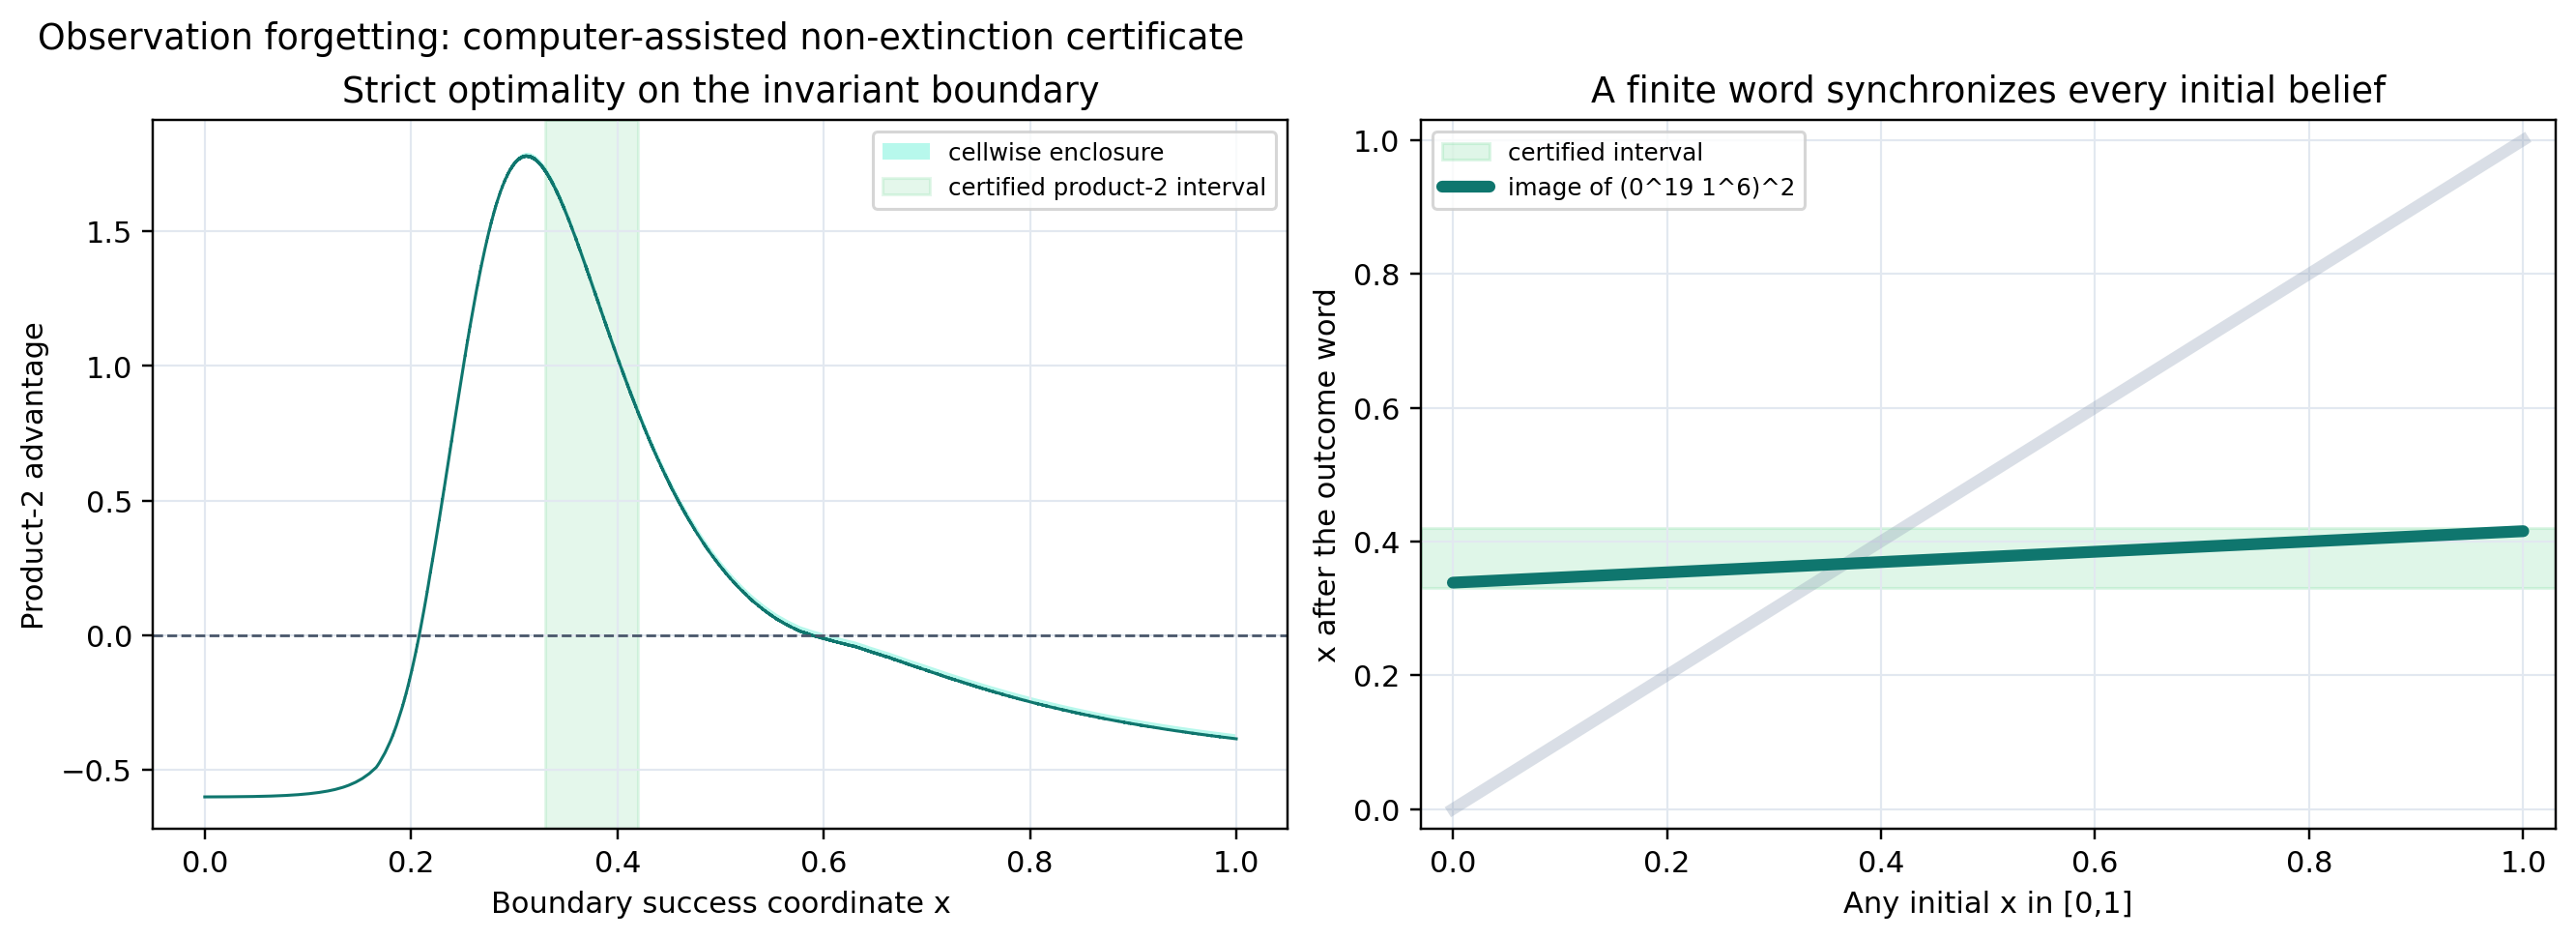
\includegraphics[width=0.96\textwidth]
    {../figures/full/diagnostics/25_observation_forgetting_nonextinction.png}
  \caption{Dos ingredientes del certificado para olvido por observación con
  $\rho=0.95$: una región con ventaja estricta y una secuencia que lleva las
  creencias maduras de vuelta a ella.}
  \label{fig:certificate}
\end{figure}

\section{Qué no debe concluirse}

\begin{itemize}
  \item Los resultados son para
  $(p_1,p_2,c_1,c_2,R,\gamma)=(0.35,0.80,0.05,0.65,1,0.98)$ y para las mallas
  y horizontes indicados.
  \item Una frecuencia tardía positiva en 5,000 periodos es evidencia de
  persistencia dentro de la simulación; por sí sola no prueba uso infinito.
  \item Una última diagonal activa numérica requiere comprobar que está lejos
  de la frontera artificial. El experimento hizo esa comparación, pero sigue
  siendo una aproximación de truncación.
  \item Las políticas con olvido son soluciones interpoladas de un estado
  continuo. Cerca de la frontera entre productos pueden existir pequeños
  desacuerdos entre mallas.
  \item Números aleatorios comunes reducen ruido al comparar métodos, pero no
  convierten una simulación en un teorema.
  \item La mayor ganancia observada en una corrida no implica que un método
  domine para otros parámetros, priors u horizontes.
\end{itemize}

\section{Conclusión}

El mensaje unificador es sencillo. El producto 2 se usa para comprar una mejor
reputación futura. Si una observación adicional deja de mover la demanda, ese
beneficio reputacional desaparece y el vendedor termina usando sólo el
producto barato. Si la demanda conserva un salto o la memoria permanece
acotada por olvido, la reputación sigue siendo sensible y la inversión en
calidad puede repetirse.

En forma resumida:
\begin{center}
\begin{tabular}{p{4.3cm}p{8.3cm}}
\toprule
Familia & Lectura principal en este experimento \\
\midrule
TS, escalado y temperatura fija & La sensibilidad se desvanece y la región de
producto 2 termina en una diagonal finita. \\
Epsilon-greedy, $\varepsilon<1$ & El salto de demanda sostiene uso recurrente
del producto 2. \\
Epsilon-greedy, $\varepsilon=1$ & La demanda no depende de reputación; no hay
razón para pagar por calidad. \\
Olvido & La memoria acotada mantiene viva la respuesta a datos recientes y se
observa inversión recurrente. \\
\bottomrule
\end{tabular}
\end{center}

\vfill
{\small\color{gris}
El reporte resume los archivos, configuraciones y resultados generados en
\texttt{Modular DP}. Las figuras conservan sus etiquetas originales en inglés
para que puedan localizarse directamente en el catálogo reproducible del
experimento.}

\end{document}
